\documentclass[10pt]{sensys-proc}

\usepackage{graphicx}
\DeclareGraphicsExtensions{.pdf,.jpg,.png}
\graphicspath{{./figures/} {./plots/}}

\usepackage{balance}
\usepackage{comment}
\usepackage{xspace}
\usepackage[export]{adjustbox}
\usepackage{wrapfig}
\newcommand{\chain}{Chain\xspace}
%\numberofauthors{1}

%\author{
%
% The command \alignauthor (no curly braces needed) should
% precede each author name, affiliation/snail-mail address and
% e-mail address. Additionally, tag each line of
% affiliation/address with \affaddr, and tag the
%% e-mail address with \email.
%\alignauthor Alice Security \\
%        \affaddr{Department of Computer Science}\\
%        \affaddr{University of Southern California}\\
%       \email{alice@example.edu}
%\alignauthor Bob Privacy \\
%    \affaddr{Networked Embedded Systems Group}\\
%    \affaddr{Swedish Institute of Computer Science}\\
%    \email{bob@example.se}
%}

\title{Chains on Threads on Tasks on Channels....}

\begin{document}

\maketitle

%Only including an abstract since it looks like the submission site wants one... 
\begin{abstract}
Killer abstract. 
\end{abstract}

\section{Introduction/Background}
  \label{sec:intro}
Intro stuff about intermittence that Brandon already knows but we should record for the
heck of it. Here's a sample citation for totally unrelated things~\cite{RC,Grace}!
  
%Sample of adding a picture across the top of a split page... 
\begin{figure*}
\centering
\begin{minipage}[b]{0.49\textwidth}
  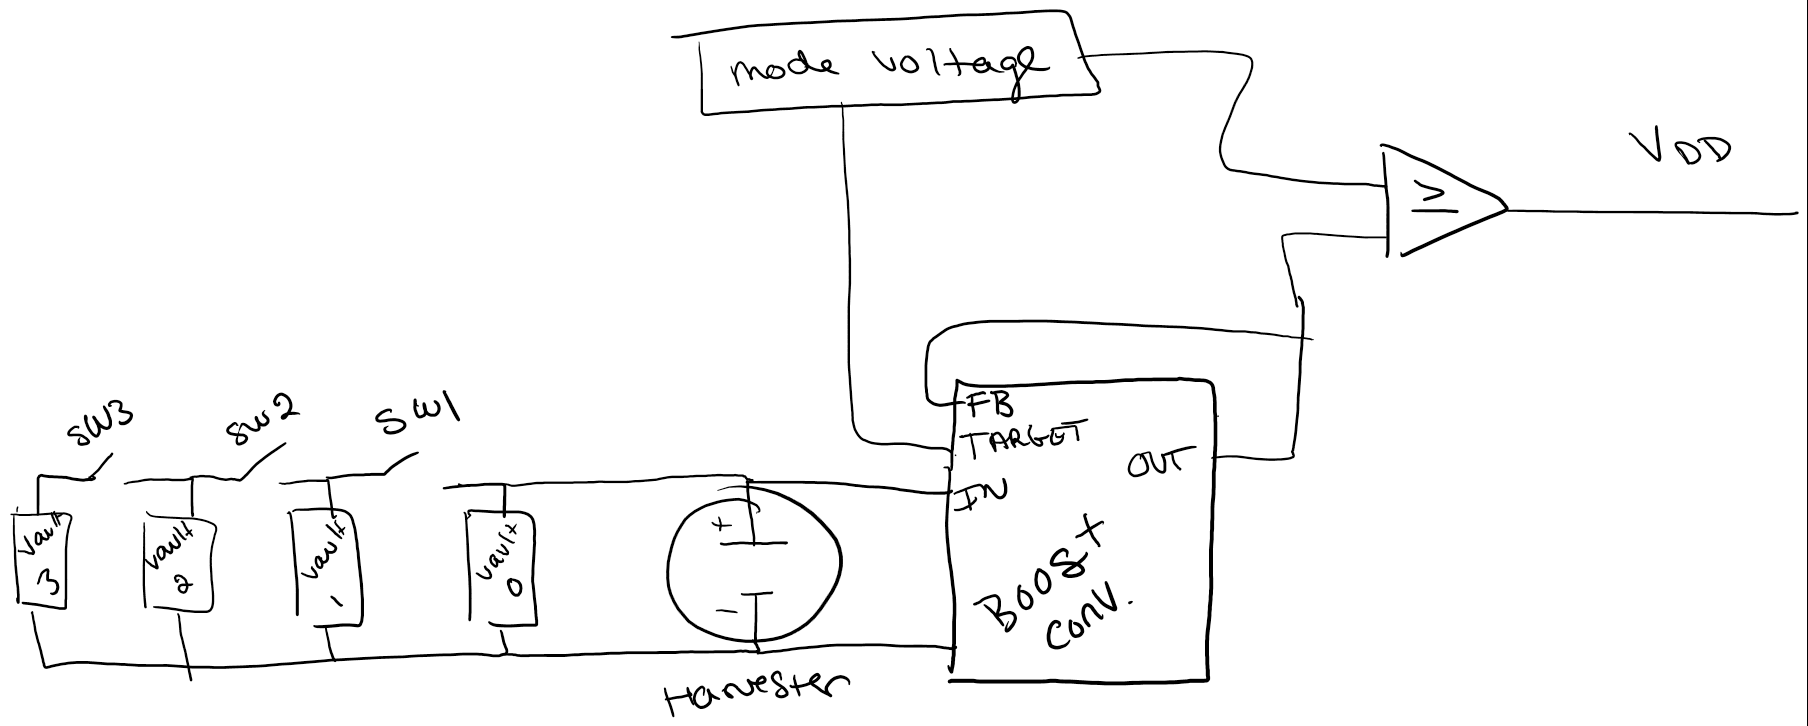
\includegraphics[width=0.95\textwidth,center]{capybara-all.png}
\caption{Capybara power system overview}\label{label-a}
\end{minipage}\hfill
\begin{minipage}[b]{0.49\textwidth}
  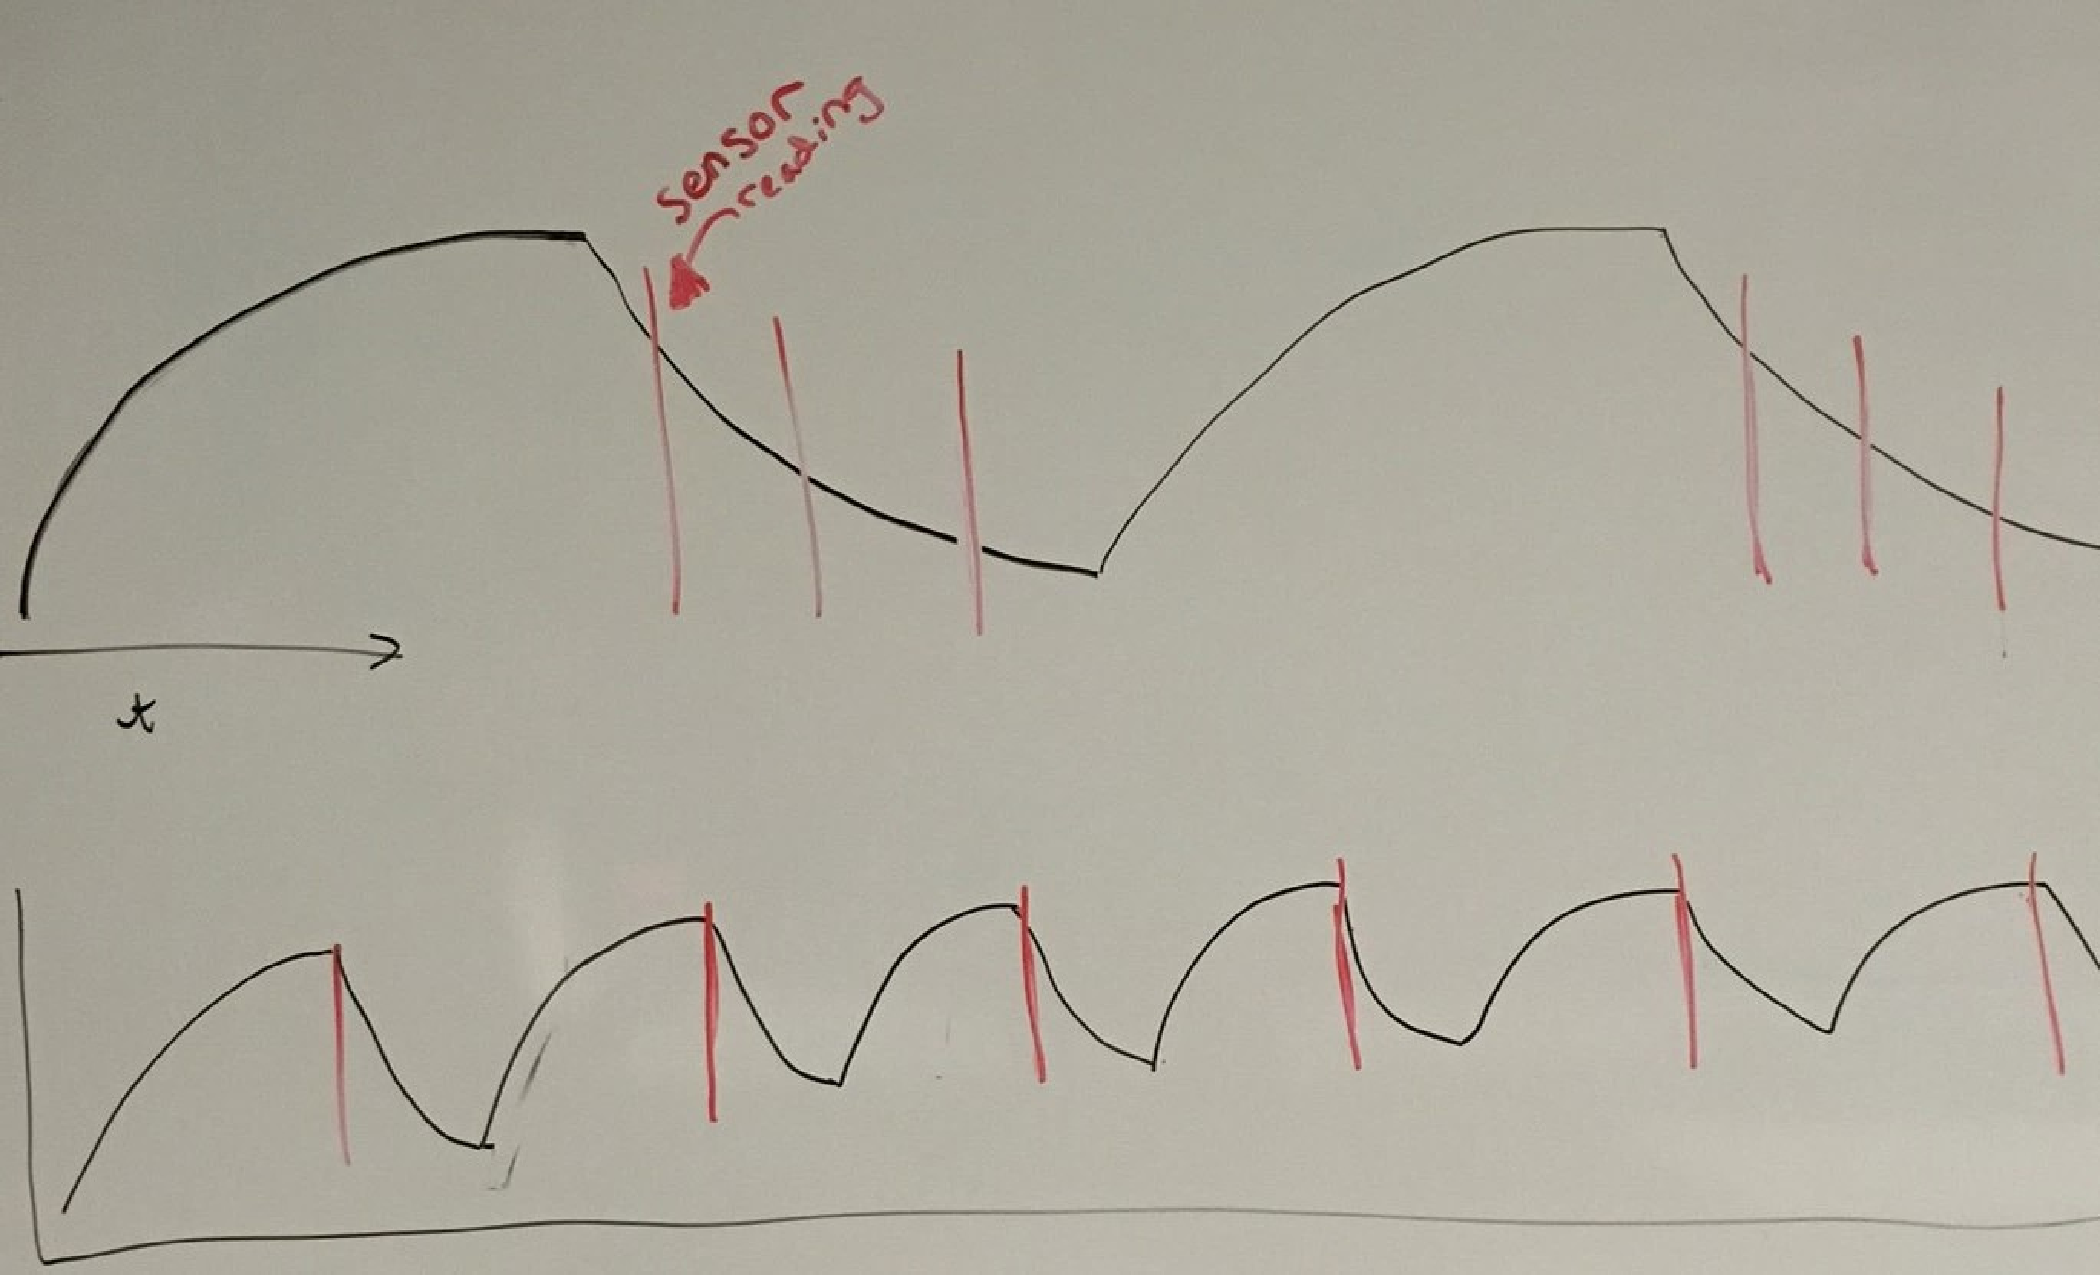
\includegraphics[width=0.95\textwidth,center]{power_modes.pdf}
\caption{Effect of different power modes}\label{label-b}
\end{minipage}
\end{figure*}

More text after the picture to show how that looks...


\section{Implementation}
We only had to break \chain a little. We promise!


\section{Results}
No really, there will be things here!


\section{Conclusion}
Multithreading in intermittence {\em is} a good idea! 


\balance
\bibliographystyle{abbrv}
\bibliography{sigproc}  % sigproc.bib is the name of the Bibliography in this case
\end{document}

